\documentclass{llncs}

\usepackage{color}
\usepackage{colortbl}
\usepackage{epsfig}
\usepackage{listings}
\usepackage{array}
\usepackage{longtable}
\usepackage{hhline}
\usepackage{cite}
\usepackage{boxedminipage}
\usepackage{graphicx}

\newcommand{\notesbox}[1]{
  \noindent\begin{center}\begin{boxedminipage}[h]{0.4\textwidth}{#1}\end{boxedminipage}\end{center}
}

\definecolor{lightgray}{gray}{.95}
\definecolor{darkgray}{gray}{.80}

\lstset{
  lineskip=0.5pt,
  basicstyle=\scriptsize,             % the size of the fonts that are used for the code
  %numbers=left,                      % where to put the line-numbers
  numberstyle=\scriptsize,            % the size of the fonts that are used for the line-numbers
  stepnumber=1,                       % the step between two line-numbers. If it is 1 each line will be numbered
  numbersep=3pt,                      % how far the line-numbers are from the code
  backgroundcolor=\color{lightgray},  % choose the background color. You must add \usepackage{color}
  showspaces=false,                   % show spaces adding particular underscores
  showstringspaces=false,             % underline spaces within strings
  showtabs=false,                     % show tabs within strings adding particular underscores
  frame=none,                         % adds a frame around the code
  tabsize=2,                          % sets default tabsize to 2 spaces
  captionpos=b,                       % sets the caption-position to bottom
  breaklines=true,                    % sets automatic line breaking
  breakatwhitespace=false,            % sets if automatic breaks should only happen at whitespace
  escapeinside={\%}{)}                % if you want to add a comment within your code
}

\hyphenation{op-tical net-works semi-conduc-tor}

\begin{document}

\title{ARC -- Automatic Repair of Concurrency Bugs}

\author{Kevin Jalbert, David Kelk, Jeremy S. Bradbury}

\institute{Software Quality Research Group\\
Faculty of Science (Computer Science)\\
University of Ontario Institute of Technology\\
Oshawa, Ontario, Canada\\
\email{\{kevin.jalbert, david.kelk, jeremy.bradbury\}@uoit.ca}}

\maketitle

\begin{abstract}

Automatic repair of single-threaded programs is being realized in practice.
Similar progress has not been made on the automatic repair of parallel
programs. We introduce a fully automated two-phase system for repairing
deadlocks and data races in parallel Java programs. The approach works on any
Java source code and requires only rudimentary test cases. Annotations, formal
specifications or other notations are not required. As only the concurrency
mechanisms are targeted the semantic meaning of the program is not changed. In
the first phase an evolutionary strategy is used to mutate the existing program
until a variant is found that fixes the deadlocks and data races. As the first
phase may introduce unneeded synchronization, a second phase attempts to
optimize performance by removing the excess synchronization without sacrificing
program correctness. We describe the approach and report on early results.

\end{abstract}

\section{Introduction}
\label{sec:introduction}

As desktop computers now ship with more than one processor, programs must
parallelize to continue to benefit from Moore's Law. Inevitably these programs
contain bugs. If fixing bugs in single-threaded programs is a difficult and
resource intensive task,  it is doubly so in multi-threaded programs.
Parallelism~\cite{SL05} introduces new classes of bugs and makes them harder to
find by having them only occur in rare execution interleavings~\cite{MQB07}.
Data races cause variables to take on unpredictable values as different threads
race to write to them while deadlocks bring part or all of a running program to
a halt.

We propose ARC (Automatic Repair of Concurrency bugs): An automatic technique
to repair deadlocks and data races in parallel Java programs. Formal
specifications, annotations and elaborate test suites are not required. Only
the Java source code and test(s) demonstrating the deadlocks and data races are
necessary. Evolutionary strategies (ES) are used to evolve variants until one
is found that fixes the bugs in question.

There has been a great deal of research in the area of search-based software
engineering~\cite{Har+10}. Furthermore, the use of heuristic search to identify
a solution fixing a bug is not a novel idea~\cite{FNWG09, AY08, Arc08, WT10,
WNLF09, WFGN10}. Our proposed approach adapts the original idea of
automatically fixing sequential programs to specifically target concurrent
software.

ES is part of the family of heuristic search algorithms. They are population-
based technique driven by mutation. Crossover and replacement are not used. All
members of the population exist throughout an invocation of the search. A
fitness function is used to evaluate each member's proposed fix. Bugs in a
concurrent program are fixed by iteratively mutating the program and evaluating
each mutation by executing the program many times. IBM's ConTest~\cite{EFN+02}
tool is used to explore different interleavings of the program under test to
increase our confidence bugs are not slipping by. Fitness improves with the
number of correct executions.

Large search spaces are a problem faced by all bug fixing techniques.
Parallelism introduces thread interleavings on top of this. A number of steps
are taken to address this issue. First, we limit the algorithm to only fixing
deadlocks and data races. Second, only the concurrency mechanisms are targeted.
Specifically, \textit{synchronize} statements are added, removed, swapped,
grown and shrunk. No other statements are affected. Third, we use a specific
set of eleven TXL~\cite{CHP91} operators based on the ConMAn
operators~\cite{BCD06} to mutate the parallel Java code.

ARC operates in two phases. In the first, synchronization blocks are added,
expanded and swapped to attempt to fix the bugs. This may add unnecessary
synchronization. If a correct program is found in phase one, a second phase
attempts to improve performance by shrinking and removing synchronization
blocks. As this can introduce data races or deadlocks, any mutant decreasing
correctness is rejected.

To the best of our knowledge there has been no previous work using evolutionary
strategies to fix bugs in concurrent software. There has been work involving
the correction of concurrency bugs using self-healing~\cite{LVK08}. From the
paper, \textit{The healing techniques based on influencing the scheduling do
not guarantee that a detected problem will really be completely removed, but
they can decrease the probability of its manifestation.} In contrast ARC is an
off-line technique that fixes bugs by modifying the source code.

The main contributions of this paper are:

\begin{itemize}

\item An algorithm to create minimal fixes for deadlocks and data races in Java
programs. Only the source code and tests demonstrating the bugs are necessary.
To the best of our knowledge this is the first approach to fix both kinds of
bugs in Java programs.

\item Methods to constrain the search space: First, by specifically targeting
synchronization mechanisms. Second, by using a limited number of TXL operators
to transform the Java source.

\end{itemize}

\section{Background}
\label{sec:background}

\begin{quote}
\textit{Some properties are difficult or impossible to encode using test cases,
such as nondeterministic properties; GenProg cannot currently repair race
conditions, for example.}~\cite{GNFW11}
\end{quote}

All of the material discussed here revolves around the topics of concurrency,
model checking, heuristic search and state-space exploration. A firm
understanding of these topics is required for various parts of the paper.

\subsection{Concurrency}
\label{sec:concurrency}

Concurrency is the act of having multiple threads executing in parallel.
Concurrent programs are able to exploit multi-core systems where threads are
distributed across each of the CPUs to increase performance. Concurrency
introduces a new class class of bugs, the \textit{heisenbugs}. Due to
concurrent access to shared memory, threads are able to cause \textit{data
races} and \textit{deadlocks}.

A \textbf{data race} has been defined as: \textit{``\ldots two or more
concurrent threads access a shared variable and when at least one access is a
write, and the threads use no explicit mechanism to prevent the access from
being simultaneous.''}~\cite{LSW07}.

A \textbf{deadlock} as: \textit{``\ldots a situation where two or more
processes are unable to proceed because each is waiting for one of the others
to do something in a deadlock cycle \ldots} For example, this occurs when a
thread holds a lock that another thread desires and vice-versa''~\cite{LSW07}.

These bugs are extremely difficult to detect due to the non-deterministic
nature of how threads are interleaved (the way the system schedules them). In
one execution a concurrency bug might occur, then a second, third and forth it
does not. Various techniques are available to detect concurrency bugs such as
static analysis~\cite{NA07,NPSG09,HP04}, stress testing~\cite{HSU03}, dynamic
analysis~\cite{JNPS09,EFN+02}, and model
checking~\cite{BHPV00,RDH03,OM03,MQB07,Holz97,JM04,HP00}.

\subsection{Evolutionary Strategies}
\label{sec:evolutionary_strategies}

ES is part of the family of heuristic search algorithms. The most commonly
referenced heuristic search technique is the genetic algorithm~\cite{GA92}. For
space reasons only the briefest outline of ES and it's place in the heuristic
search family is given.

A standard genetic algorithm is population based, uses mutation, crossover and
a fitness function to evolve solutions to problems. A proposed solution to the
problem is encoded as a member of the population. Each member is evaluated by a
fitness function. The more fit a member solution is, the greater the chance it
will pass it's genetic material (solution) on to the next generation.
\textit{Selection pressure preferentially selects better solutions.} Crossover
mixes these solutions to produce new ones while mutation injects fresh
information in to the population so it doesn't become stagnant.

ES is a simpler form of search than a genetic algorithm. A population of
proposed solutions is generated and mutated each generation. Crossover and
selection aren't used, so the same population exists throughout the evolution.
Every members fitness is evaluated every generation. It ends when a
predetermined fitness is reached or after a set number of generations have
passed.

Why use mutation only? Sometimes it is unclear how to use crossover. For
example, if the member solutions are Java programs, how does one ensure that
when putting two halves of different programs together the resulting program is
correct, makes sense or even compiles?

\section{Related Works}
\label{sec:related_works}

There are a number of approaches to automatically hide or fix bugs in programs.
Co-evolutionary competition between programs with bugs and test cases is used
in~\cite{AY08, Arc08, WT10}. Both approaches require formal specifications and
both use genetic programming to evolve fixes. Co-evolution is used to cause
competition between the evolving fixes and test cases. In both cases the
resulting framework is tested only against a toy sorting algorithm with mixed
success. The untargeted nature of the fixing process is the largest limitation.
No effort is made to constrain the large search space of the problem.

Significant improvements are made in~\cite{FNWG09, WNLF09, NWLF09, WFGN10,
GNFW11}. Formal specifications are no longer required. Instead, test cases are
used to demonstrate the bug and describe the desired functionality that must be
preserved. To address the limitations of the previous approach they introduce
two innovations: First, they assume the bug is written correctly in another
part of the program. Second, they determine the error path on which the bug
occurs and target those statements specifically for repair. Together these
additions constrain the state space enough that the framework can fix real bugs
in real programs.

Similar to the work done here,~\cite{KLT+07, LVK08} uses ConTest to heal data
races. From their paper, \textit{``Healing concurrency problems is about
limiting or changing the probability of interleaving, such that bugs will be
seen less.''} In contrast, our approach uses ConTest in a framework that fixes
both deadlocks and data races.

A framework is created in~\cite{CB05} to ``repair'' buffer overflow attacks.
When one is identified, the program state is reset to what it was before the
attack. The attack packet is discarded then the program continues running. As
in the previous approach the goal is to hide the problem, not fix it.

SAT solving is used in~\cite{AY07}  to repair shared memory concurrent programs
``w.r.t. CTL specifications'' where processes atomically read, write one shared
variable at a time. All that is required is the concurrent program and a
specification in modal or temporal logic. It is unclear if the fix is applied
to the program or the specification of the program.

\section{Motivating Problem}
\label{sec:motivation}

Concurrency bugs are difficult to detect and fix. Many tools exist that
identify concurrent bugs. The identification of a problem is often not enough
as multiple code fragments are involved, possibly in different units with
differently named variables. In this ambiguous scenario the appropriate fix is
not always clear. There has been work in concurrency anti-patterns that provide
a definition, problem, context and solution for concurrency
bugs~\cite{BJ09,FKLV12}.

In the left part of Fig.~\ref{fig:fixed_sample_datarace} the \texttt{read} and
\texttt{write} method access a shared variable. A very simple data race exists
because there is no atomic access to the \texttt{data} variable during the
reading or writing. Both methods are involved in the data race, and it is
because of the interactions between these methods the data race is possible. A
solution involves synchronizing both accesses (Right part of
Fig.~\ref{fig:fixed_sample_datarace}). Synchronizing one method alone does not
fix the bug.

The solution in the right part of Fig.~\ref{fig:fixed_sample_datarace} is far
from ideal. It forces other threads to wait unnecessarily while the write
method works in the loop and database sections. An optimization is to shrink
the critical region (the synchronized statements) to only guard access to the
shared variable (as shown in Fig.~\ref{fig:optimized_sample_datarace}).

\begin{figure}[h]
\begin{minipage}{5cm}
\footnotesize{\textbf{Buggy Program:}}
\begin{lstlisting}[language=Java, morekeywords={synchronize}]
write(int var1){
  ... // Expensive loop
  data = var1;
  ... // Database query
}

int public read(){
  return data;
}
\end{lstlisting}
\end{minipage}\hfill
\begin{minipage}{5cm}
\footnotesize{\textbf{Fixed Program:}}
\begin{lstlisting}[language=Java, morekeywords={synchronize}]
synchronize write(int var1){
  ... // Expensive loop
  data = var1;
  ... // Database query
}

int synchronize read(){
  return data;
}
\end{lstlisting}
\end{minipage}
\caption{A developer first synchronizes the \texttt{read} function, yet the bug
still exists. Synchronizing the \texttt{write} method as well fixes it.}
\label{fig:fixed_sample_datarace}
\end{figure}

\begin{figure}[t]
\begin{minipage}{5cm}
\footnotesize{\textbf{$1^{st}$ Optimization on Fix:}}
\begin{lstlisting}[language=Java, morekeywords={synchronize}]
public write(int var1){
  ... // Expensive loop
  synchronized(this){
    data = var1;
    ... // Database query
  }
}

int synchronize read(){
  return data;
}
\end{lstlisting}
\end{minipage}\hfill
\begin{minipage}{5cm}
\footnotesize{\textbf{$2^{nd}$ Optimization on Fix:}}
\begin{lstlisting}[language=Java, morekeywords={synchronize}]
public write(int var1){
  ... // Expensive loop
  synchronized(this){
    data = var1;
  }
  ... // Database query
}

int synchronize read(){
  return data;
}
\end{lstlisting}
\end{minipage}
\caption{A developer shrinks the critical region to exclude the expensive loop.
They shrink the critical region again to exclude the database query as a
further optimization.}
\label{fig:optimized_sample_datarace}
\end{figure}

From a developer's standpoint there is a lot of work involved in creating a fix
for parallel bugs as multiple, unrelated changes are not uncommon. Two changes
were required to functionally fix the example program. Two additional changes
were required to improve the non-functional performance.

Automated tools in software testing and debugging are needed as they have the
potential to reduce the vast amount of resources spent on software testing
(upwards to \$59.5 billion)~\cite{RTI02}. ARC provides an automated approach to
fixing the \textit{functionality}, and then optimizing the \textit{non-
functional} performance of programs with deadlocks and data races.

\section{ARC's Approach}
\label{sec:approach}

ARC aims to automatically repair concurrency bugs like the one presented in
Sect.~\ref{sec:motivation}. A high-level overview of ARC's approach is
presented in Fig.~\ref{fig:process}. There are two inputs to ARC: A buggy
concurrent Java program and a JUnit test suite. The test suite is necessary as
it acts like an oracle to determine if the bug still exists in the program. One
limitation of ARC (and of other automatic bug fixing techniques mentioned in
Sect.~\ref{sec:related_works}) is that it can only fix bugs detectable by the
test suite.

\begin{figure}[h]
  \centering
  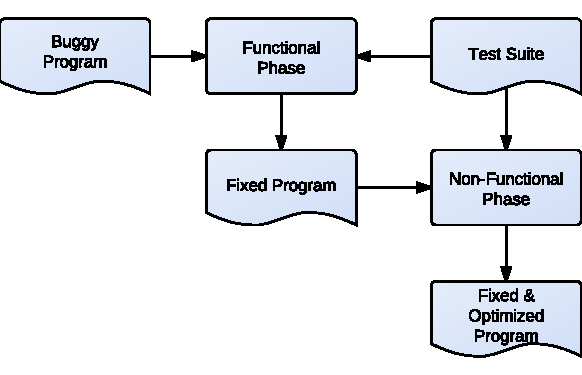
\includegraphics[width=7.0cm]{figures/process.pdf}
  \caption{High Level Overview of ARC's Repair and Optimization Process}
  \label{fig:process}
\end{figure}

ARC's complete approach is accomplished in two phases, the \textit{Functional
Phase} and the \textit{Non-Functional Phase}. Both are similar in terms of the
steps they follow, with slight variations to accomplish different goals. The
first phase attempts to fix the buggy program while the second attempts to
optimize its performance.

The next sections detail each step of the two phases as shown in
Fig.~\ref{fig:phases_internals}, with the differences between phases being
indicated. The key aspect of ARC's approach fall in the mutation and evaluation
steps.

\begin{figure}[h]
  \centering
  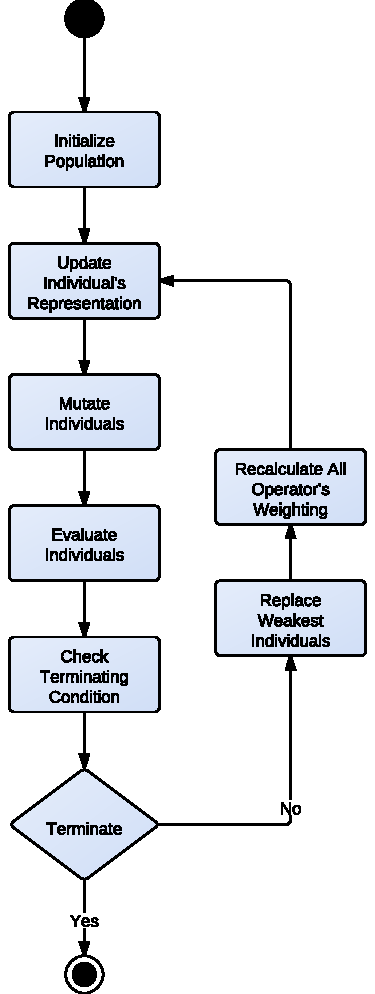
\includegraphics[width=4.50cm]{figures/phases.pdf}
  \caption{Internal View of ARC's Phases}
  \label{fig:phases_internals}
\end{figure}

\subsection{Initialize Population}
\label{sec:initialize_population}

ARC begins each phase first by initializing the population of individuals. This
involves creating a copy of the program for each individual that is mutated by
the ES. For the non-functional phase ARC has already produced the fixed
program so each individual receives a copy of the fixed program to optimize.

\subsection{Generate Mutants and Update Individual's Representation}
\label{sec:update_individual_representation}

For each individual the previous generation's code is used to generate all
possible mutations that can be applied for this generation. This step generates
all possible mutants for each individual, though the actual mutation is applied
in the next step. Internally ARC keeps track of the mutants using a
representational form as shown in Table~\ref{tbl:individual_representation}. As
there exists multiple types of mutations, individuals are represented using a
2-dimensional array of the mutation operators and the number of mutation
instances generated.

\begin{table}[h]
\begin{center}
\caption{An example representation of an individual, each 0 represents an
instance of that mutation type that has been generated. It is possible for up
to $n$ mutation operators with no-limit to the number of instances per
operator.}
\begin{tabular}{|l|l|}
\hline
\textbf{Operator} & \textbf{Instances}\\
\hline
Mutation 1 & 0\\
\hline
Mutation 2 & 0 0 0\\
\hline
Mutation 3 & --\\
\hline
\ldots & \ldots\\
\hline
Mutation $n$ & 0 0\\
\hline
\end{tabular}
\label{tbl:individual_representation}
\end{center}
\end{table}

The set of mutation operators ARC uses are listed in Table~\ref{tbl:operators},
each operator can aid in repairing and/or optimizing the program. The majority
of the ARC mutation operators have been derived from the ConMAn
operators~\cite{BCD06}. These operators work by searching for a pattern within
the source code and then transforming it according to a set of rules. An
example of the EXSB mutation operator is shown in Fig.~\ref{fig:EXSB_example}.

\begin{table}[h]
\caption{Set of mutation operators used by ARC. Each mutation operator is
active during the indicated phases.}
\begin{center}
\begin{tabular}{|l|l|c|c|}
\hline
\textbf{Operator} & \textbf{Acronym} & \textbf{Functional} & \textbf{Non-Functional}\\
\hline
Add synch. around synch. & ASAS & $\surd$ &\\
\hline
Add synch. around variable & ASAV & $\surd$ &\\
\hline
Add synch. in method header & ASIM & $\surd$ &\\
\hline
Add synch. around method & ASM & $\surd$ &\\
\hline
Change synch. order & CSO & $\surd$ &\\
\hline
Expand synch. before & EXSB & $\surd$ &\\
\hline
Expand synch. after & EXSA & $\surd$ &\\
\hline
Remove synch. around synch. & RSAS & $\surd$ & $\surd$\\
\hline
Remove synch. around variable & RSAV & $\surd$ & $\surd$\\
\hline
Remove synch. in method header & RSIM & $\surd$ & $\surd$\\
\hline
Remove synch. around method & RSM & $\surd$ & $\surd$\\
\hline
Shrink synch. before & SHSB & & $\surd$\\
\hline
Shrink synch. after & SHSA & & $\surd$\\
\hline
\end{tabular}
\label{tbl:operators}
\end{center}
\end{table}

\begin{figure}[h]
\vspace{2mm}
\begin{minipage}{5cm}

\footnotesize{\textbf{ Program $P$:}}
\begin{lstlisting}[language=Java, morekeywords={synchronize}]
  ...
  obj.write(var1);
  synchronized(lock){
    myHash.remove(var1);
  }
\end{lstlisting}
\end{minipage}\hfill
\begin{minipage}{5cm}
\footnotesize{\textbf{ Program $P'$:}}
\begin{lstlisting}[language=Java, morekeywords={synchronize}]
  ...
  synchronized(lock){
    obj.write(var1);
    myHash.remove(var1);
  }
\end{lstlisting}
\end{minipage}

\caption{An example of the EXSB (expand synchronization before) mutation
operator.}
\label{fig:EXSB_example}
\end{figure}

As ARC mutates synchronization aspects of programs, the mutations themselves
can alter the appearance of future mutations. This causing the search space of
possible mutations to potentially changes in every generation. Thus ARC must
update the representation according to the latest state of the program's source
code each generation.

\subsection{Apply a Mutation to an Individual}
\label{sec:mutate_individuals}

Once all mutations are generated for each individual ARC selects a type of
mutation and then an instance of that from the individual's representation. The
selected mutation of the previous generation's code then acts as the current
generation's code. ARC at this point will re-compile the project to ensure that
the mutation consists of valid syntax. In the situation that the compilation
fails another mutation and instance is selected until a valid combination is
found.

ARC can leverage historical information about previous evaluations with the
mutation operators along with information about the current dominating bug type
found during testing. These two pieces of data add weight to operators
that have been successful in the past, as well as to select operators that
appear to reduce the occurrences of either deadlocks or data races more often.
This heuristic is further detailed in
Sect.~\ref{sec:recalculate_operator_weighting}. Currently, ARC randomly select
an instance of the operator to accept as our final mutation for that
individual.

\subsection{Evaluate Individuals}
\label{sec:evalute_individuals}

A mutation may be beneficial, destructive or benign. We must evaluate it to
determine the effect on the program. A key problem is the unpredictability of
thread interleavings. If a concurrency bug appears only rarely, how can we gain
confidence that a proposed fix actually works? ARC uses IBM's ConTest
tool~\cite{EFN+02} to instrument the project by injecting noise into the
program. The injected noise causes threads to yield, sleep and wait randomly,
effectively causing an execution of the program to explore a diverse set of
scheduled interleavings. By running ConTest (the instrumented version of the
program) multiple times we gain more confidence that a larger set of the
interleavings are explored. Running the instrumented program multiple times is
the most time consuming aspect of ARC.

In the first phase ARC attempts to repair the buggy program, thus the fitness
is determined by the number of successful ConTest executions. More successes
translates in to higher fitness value. We consider timeouts as a positive
factor in the fitness function as it could either result in a deadlock or a
successful execution given more time. We do weight timeouts less than a
successful execution as it could still result in a deadlock.
Figure~\ref{fig:functional_fitness} displays the first phase's fitness
function.

\begin{figure}[h]
\begin{footnotesize}
\begin{center}
$functional\ fitness(P) = (s \times sw) + (t \times tw)$
\end{center}
\end{footnotesize}
\begin{scriptsize}
\begin{center}
$s = \#\ of\ successful\ executions$ \\
$sw = success\ weighting$ \\
$t = \#\ of\ timeout\ executions$ \\
$tw = timeout\ weighting$
\end{center}
\end{scriptsize}
\caption{Fitness Function for Functional Phase}
\label{fig:functional_fitness}
\end{figure}

If ARC finds an individual that achieves 100\% successful executions during the
first phase, we need to ensure it is truly a fix. It is possible that a
proposed solution could still contain a concurrency bug that escaped detection
because the bug exhibiting interleavings was not encountered. Our safeguard is
to run ConTest an additional number of times (some multiple of the previous
number of runs). If the fix still holds even after this validation we feel
confident the solution is indeed a true solution. If any of the additional
executions fail, the proposed fix is rejected and the evolutionary process
continues.

Once a fix is found ARC begins the second phase, to optimize the found
solution. We utilize a new fitness function that combines the real time
required for an execution as well as the number of voluntary context switches
made. The real time taken is an obvious choice to use to measure the
performance of the program, while the number of voluntary context switches
gives us an indication on the amount of thread switching. By minimizing
unnecessary synchronization the number of context switches should decrease
along with the real time taken as seen in Fig.~\ref{fig:nonfunctional_fitness}.
Baseline time and context switches are generated from the newly fixed program
by running it a large number of times and averaging the values acquire. This
baseline is then used in the fitness function to evaluate relative improvements
from the fixed unoptimized program. Note that the fitness function adjusts
based on the significance and uncertainty of both variables (to be fair in
situations where either variable is under-represented).


\begin{figure}[h]
\begin{footnotesize}
\begin{center}
$non-functional\ fitness(P) = \frac{worst\ score}{[sig_t \times unc(t)] + [sig_c \times unc(c)]}$
\end{center}
\vspace{0.1cm} \textit{Where:} \vspace{0.1cm}
\end{footnotesize}
\begin{scriptsize}
\begin{center}
$unc(x) = \frac{(x_{max} - x_{min})}{x_{avg}}$ \\ \vspace{0.2cm}
$
  sig_t = \left\{
  \begin{array}{l l}
    t/c & \quad if\ t\ > c \\
    c/t & \quad if\ c\ > t \\
  \end{array} \right.
$ \\ \vspace{0.2cm}
$
  sig_s = \left\{
  \begin{array}{l l}
    c/t & \quad if\ t\ > c \\
    t/c & \quad if\ c\ > t \\
  \end{array} \right.
$ \\
\end{center}
\end{scriptsize}
\caption{Fitness Function for Non-Functional Phase}
\label{fig:nonfunctional_fitness}
\end{figure}

Removing and reducing synchronization runs the risk of introducing new bugs
into the program. Before every non-functional phase evaluation we need to
ensure that no bugs are present, thus we re-run the functional phase's
evaluation with the multiplier on the number of runs. If any deadlocks or data
races are encountered the proposed optimization is rejected and this individual
is reset to the previous generation. After ARC validates the proposed
optimization additional runs are conducted without using ConTest (avoids the
inclusion of random noise) to obtain the values required for the non-functional
fitness function.

As it is not clear when an individual's program reaches its maximum
optimization -- and there is no a-priori way to know this, ARC runs phase two
for it's full allotment of generations. At the end it outputs the member
program with the highest non-functional fitness (from any generation) as the
final optimized fix.

\subsection{Check Terminating Condition}
\label{sec:check_terminating_condition}

Each phase continues to evolve and evaluate individuals until some terminating
condition is met. The following conditions are for the functional phase: A
solution is found (100\% successful executions in validation) or no solution is
found within the generational limit. The following conditions are for the non-
functional phase: The population has converged (no improvement has been seen in
$x$ generations), no more mutations are generated, or the generational limit is
hit.

\subsection{Replace Weakest Individuals}
\label{sec:replace_weakest_individuals}

With any evolutionary algorithm it is entirely possible for an individual to
stray down a path leading to little or no improvement. To encourage individuals
to explore more fruitful areas of the state space we employ a replacement
strategy that replaces the lower $w$ percentage of individuals with a random
individual from the upper $x$ percent. These replacements only occur after an
individual has underperformed for $y$ generations. We believe the correct
program isn't very far away in the state space from the original buggy program.
Therefore we also provide a change for an under-performing individual to reset
back the initial state to allow the individual to explore from the starting
point again.

\subsection{Recalculate All Operator's Weighting}
\label{sec:recalculate_operator_weighting}

ARC utilizes a heuristic approach to select the mutation operator in the
mutation step. A sliding window of $n$ generations is used to determine the
success of previously used mutation operators. Operators that improve fitness
are weighted more heavily and are more likely to be selected. A sliding window
is used to prevent dominance of operators and to allow for flexibility in
changing weighting based on recent history. The weighting is designed to ensure
the chance of selecting an operator is always greater than zero regardless of
performance. To ensure this approach is up to date the current weighting for
each operator is recalculated based on the new feedback received from the
population. In the functional phase we consider a separate weighting for data
races and deadlocks to remain accurate in the use of this heuristic.

\section{Experiments}
\label{sec:experiments}

Due to the ARCs heuristic nature it is entirely possible for a program to
perform better or worse then it did originally. We are interested in both ARCs
ability to find fixes and ARCs effect on performance of solutions found.

ARC is not a quick process. Executing ConTest (population $\times$ generations
$\times$ \# runs) times alone can take significant resources. Suffice it to say
ARC is an off-line process one could run over night.

\subsection{Experimental Setup}
\label{sec:experimental_setup}

Programs ARC is evaluated against come from the IBM Concurrency
Benchmark~\cite{EHSU06}. This set of programs is rather small yet demonstrate a
variety of concurrent bug types. None of them contain the required JUnit test
suite. They were manually created without altering the programs and their
bugs\footnote{One incorrect program was fixed so that it properly exhibited its
concurrency bug.}. Details on the programs are presented in
Table~\ref{tbl:used_programs}.

% TODO Figure out the bug pattern of the follow programs

\begin{table}[h]
\caption{The set of programs used to evaluate ARC. The test suite for each
program is excluded from these values.}
\begin{center}
\begin{tabular}{|l|r|r|l|l|}
\hline
\textbf{Program} & \textbf{SLOC} & \textbf{Classes} & \textbf{Bug Type} & \textbf{Bug Pattern}\\
\hline
account & 165 & 3 & Data Race & blah\\
\hline
accounts & 75 & 2 & Data Race & blah\\
\hline
airline & 93 & 1 & Data Race & blah\\
\hline
allocation & 165 & 3 & Data Race & blah\\
\hline
bubble & 246 & 4 & Data Race & blah\\
\hline
bubblesort2 & 104 & 2 & Data Race & blah\\
\hline
buffer & 319 & 5 & Data Race & blah\\
\hline
bufwriter & 170 & 5 & Deadlock & blah\\
\hline
deadlock & 109 & 2 & Deadlock & blah\\
\hline
lottery & 157 & 2 & Data Race & blah\\
\hline
mergesort & 281 & 2 & Data Race & blah\\
\hline
pingpong & 143 & 4 & Data Race & blah\\
\hline
\end{tabular}
\label{tbl:used_programs}
\end{center}
\end{table}

ARC was designed to be flexible in terms of the parameters that can be
configured. Table~\ref{tbl:used_parameters} lists and describes each parameter,
including the values selected for evaluation. Values were selected based on our
experience with ARC.

% TODO Maybe reduce this to the common ES parameters?

\begin{table}[h]
\caption{The set of parameters that ARC uses along with their descriptions and
used values for the experimentations.}
\begin{center}
\begin{tabular}{|p{3cm}|p{10cm}|r|}
\hline
\textbf{Parameter} & \textbf{Description} & \textbf{Value}\\
\hline
Project Test Mb & The amount of memory allocated for the testing & 2000\\
\hline
ConTest Runs & The number of test suite executions performed in the functional phase & 10\\
\hline
ConTest Validation Multiplier & A multiplier for the number of runs when validating the functionality & 15\\
\hline
ConTest Timeout Multiplier & A multiplier for the dynamically acquire average execution time that determines the length of time before a timeout occurs & 300\\
\hline
Evolution Generations & The maximum number of generations that can occur within each phase & 30\\
\hline
Evolution Population & The size of the population for the evolutionary strategy, a collection of individuals & 30\\
\hline
Evolution Replace Lowest Percent & The scoring individuals that reside below the given percent of the population will be replaced/restarted & 10\\
\hline
Evolution Replace With Best Percent & The replaced individuals will be replaced with the best individual of the population with the given percent, otherwise it is restarted & 75\\
\hline
Evolution Replace After Minimum Turns & The minimum number of turns an individual must be under-performing before being considered for replacement & 3\\
\hline
Evolution Replace Interval & The replacement of lowest individuals only occurs on the specified generational intervals & 5\\
\hline
Dynamic Ranking Window & The number of generations that are considered (in a sliding window fashion) when re-evaluating the weighting of mutation operators in terms of their successes & 5\\
\hline
Success Weight & The weighting applied for successful executions during the functional phase's evaluation & 100\\
\hline
Timeout Weight & The weighting applied for timeout executions during the functional phase's evaluation & 50\\
\hline
Generational Improvement Window & This specifies the size of the sliding window that check for convergence of the population & 10\\
\hline
Average Fitness Min Delta & When checking for convergence this represents the minimum acceptable delta for the average fitness of the population & 0.01\\
\hline
Best Fitness Min Delta & When checking for convergence this represents the minimum acceptable delta for the best fitness of the population & 1\\
\hline
\end{tabular}
\label{tbl:used_parameters}
\end{center}
\end{table}

\subsection{Experimental Results}
\label{sec:experimental_results}

Each program was run through ARC a total of 10 times using the parameters
described in Table~\ref{tbl:used_parameters}. The results of each program is
summarized in Table~\ref{tbl:summary_results}.

% TODO Redo this table, and exclude the non-functional aspects of it and enumerate (somehow) the results instead of using ranges

\begin{table}[h]
\caption{Summary of the results of running the programs
(Table~\ref{tbl:used_programs}) through ARC 10 times.}
\begin{center}
\begin{tabular}{|p{2cm}|p{0.6cm}|p{1.75cm}|p{2cm}|p{2cm}|p{2cm}|p{2cm}|}
\hline
\textbf{Program} & \textbf{\% of Fixes} & \textbf{Range of Fix Containing Generation} & \textbf{Range of Original's Execution Time (s)} & \textbf{Range of Solution's Execution Time (s)} & \textbf{Range of Original's \# of Context Switches} & \textbf{Range of Solution's \# of Context Switches}\\
\hline
account & 0.6 & [3--17] & [0.10--0.14] & [0.9--0.12] & [73--97] & [60--81]\\
\hline
accounts & 0.6 & [3--17] & [0.10--0.14] & [0.9--0.12] & [73--97] & [60--81]\\
\hline
airline & 0.6 & [3--17] & [0.10--0.14] & [0.9--0.12] & [73--97] & [60--81]\\
\hline
allocation & 0.6 & [3--17] & [0.10--0.14] & [0.9--0.12] & [73--97] & [60--81]\\
\hline
bubble & 0.6 & [3--17] & [0.10--0.14] & [0.9--0.12] & [73--97] & [60--81]\\
\hline
bubblesort2 & 0.6 & [3--17] & [0.10--0.14] & [0.9--0.12] & [73--97] & [60--81]\\
\hline
buffer & 0.6 & [3--17] & [0.10--0.14] & [0.9--0.12] & [73--97] & [60--81]\\
\hline
bufwriter & 0.6 & [3--17] & [0.10--0.14] & [0.9--0.12] & [73--97] & [60--81]\\
\hline
deadlock & 0.6 & [3--17] & [0.10--0.14] & [0.9--0.12] & [73--97] & [60--81]\\
\hline
lottery & 0.6 & [3--17] & [0.10--0.14] & [0.9--0.12] & [73--97] & [60--81]\\
\hline
mergesort & 0.6 & [3--17] & [0.10--0.14] & [0.9--0.12] & [73--97] & [60--81]\\
\hline
pingpong & 0.6 & [3--17] & [0.10--0.14] & [0.9--0.12] & [73--97] & [60--81]\\
\hline
\end{tabular}
\label{tbl:summary_results}
\end{center}
\end{table}


\section{Challenges}
\label{sec:challenges}

ARC has three major challenges to face:

\textbf{Large Solution Space}: In Arcuri's approach~\cite{AY08}, they were
considering the whole program along with a large set of mutations. When
combined with a large number of places to apply them it creates an extremely
large search space for finding the solution. In ARC we are only considering
concurrency bugs and are only mutating concurrency mechanisms with concurrency
mutation operators. Inherently ARC has a much smaller search space to explore
to find a fix.

The search space can be reduced even further by considering only the mutation
falling on the error path (Used in Weimer's approach~\cite{GNFW11}) or even by
using external detection tools for potential a locational where the bug might
be residing. These two suggestions are considered for future work to minimize
the solution space.

\textbf{Dependence on Test Suite}: ARC depends on a minimal test suite for the
program being repaired. In both Arcuri's and Weimer's
approach~\cite{AY08,GNFW11} the test suites are used to both guard the
program's functionality and to indicate a bug is present. ARC requires a test
suit to exhibit the bug. ARC currently has no solution for dealing with bugs
that occur outside of the test suite's coverage. Arcuri's and Weimer's
approaches also has no solution for this.

There has been some work that attempts to co-evolve the test suite at the same
time to help check for new situations~\cite{WT10}. We assume the
test suite is comprehensive enough to detect all bugs. ARC will eventually only
consider using mutation operators that fall within the coverage of the test
suite to avoid introducing new bugs the test suite cannot detect.

\textbf{Program Readability}: Automatically fixing and optimizing a program
raises the question of source readability. None of the related work considers
the readability of their fixes. This is a concern as developers want to
understand the fix as well. Posnett et. al.~\cite{PHD11} use the following
metrics to estimate readability:

\begin{itemize}
  \item Moving lines around does not affect the program's readability
  \item The addition of existing tokens does not reduce the program's
readability as much as adding new unique statements
\end{itemize}

ARC simply adds, removes manipulates synchronization statements. In most cases
there will already tokens regarding synchronization within the program. Thus,
the addition of new synchronization does not reduce the program's readability
that much. For the mutations that manipulate the synchronization statements ARC
is effectively moving lines around, which does not reduce the program's
readability.

% Readability metrics for programs fixed by ARC are collected in
% Table~\ref{tbl:readability}.
% \ldots % TODO

% \begin{table}[h]
% \caption{The program readability values from the buggy program to the fixed
% program to the optimized program.}
% \begin{center}
% \begin{tabular}{|l|p{2cm}|p{2cm}|p{2cm}|p{2cm}|p{2cm}|}
% \hline
% \textbf{Program} & \textbf{Buggy Program's Readability} & \textbf{Fixed Program's Readability} & \textbf{Optimized Program's Readability} & \textbf{Change from Buggy to Fixed} & \textbf{Change from Fixed to Optimized}\\
% \hline
% account & 100 & 110 & 105 & +10\% & -4.6\%\\
% \hline
% accounts & 100 & 110 & 105 & +10\% & -4.6\%\\
% \hline
% airline & 100 & 110 & 105 & +10\% & -4.6\%\\
% \hline
% allocation & 100 & 110 & 105 & +10\% & -4.6\%\\
% \hline
% bubble & 100 & 110 & 105 & +10\% & -4.6\%\\
% \hline
% bubblesort2 & 100 & 110 & 105 & +10\% & -4.6\%\\
% \hline
% buffer & 100 & 110 & 105 & +10\% & -4.6\%\\
% \hline
% bufwriter & 100 & 110 & 105 & +10\% & -4.6\%\\
% \hline
% deadlock & 100 & 110 & 105 & +10\% & -4.6\%\\
% \hline
% lottery & 100 & 110 & 105 & +10\% & -4.6\%\\
% \hline
% mergesort & 100 & 110 & 105 & +10\% & -4.6\%\\
% \hline
% pingpong & 100 & 110 & 105 & +10\% & -4.6\%\\
% \hline
% \end{tabular}
% \label{tbl:readability}
% \end{center}
% \end{table}

\section{Threats to Validity}
\label{sec:threats}

% TODO

\section{Future Work}
\label{sec:future_work}

Currently ARC mutates all variables in the program under test. Ideally it
should target only those involved in concurrency. We believe there are off-the-
shelf solutions that ARC can utilize to give it this capability, similar
to~\cite{CM08, HP00}.

Targeting the variables, functions and classes on the error path is another
feature we would like to add. It has shown great success in helping to isolate
and automatically fix bugs in single-threaded programs~\cite{FNWG09, NWLF09,
WFGN10, GNFW11}. We believe it will do the same for multi-threaded programs.

Generalizing the TXL operators is also important. Currently the add
synchronization around synchronization operator (ASAS) for example, only adds
\texttt{synchronize(this) \{\ldots\}} to the Java source. When the analysis of
the previous two paragraphs are implemented the operators need to be updated to
work with them.

We also plan to experiment with new operators. Potential additions include
splitting or merging synchronization blocks and changing the argument in the
synchronize call.

Many new concurrency structures were introduced in Java 5. Expanding ARC's
operators to deal with new anti-patterns~\cite{BJ09, BCD06} gives ARC the
ability to fix additional types of bugs.

\section{Conclusion}
\label{sec:conclusion}

Little work has been done on automatically fixing parallel programs. We
introduced ARC -- a framework that automatically fixes deadlocks and data races
in parallel Java programs. It uses an evolutionary algorithm operating in two
phases. Bugs are fixed in the first phase, then concurrency is optimized in the
second.

Experiments were conducted to evaluate ARC using a set of 12 programs found in
a concurrency benchmark. The results indicate that ARC is \ldots % TODO

\bibliographystyle{splncs03}
\bibliography{SSBSE2012}

\end{document}
